\documentclass[11pt,a4paper]{scrartcl}

\usepackage[ngerman,english]{babel}
\usepackage{graphicx}
\graphicspath{{pics/}}

\title{Hair Simulation with OpenCL}
\author{Etienne Gramlich \& Heiko Ettwein}


\begin{document}
\maketitle
\tableofcontents
\newpage
\pagenumbering{arabic}

\section{Introduction}
This is a project for the course GPU programming at HTWG Konstanz.

\subsection{Project Description}
This is a hair simulation that runs on the GPU.
The hairs are made of nodes and links between them, then forces (i.e. wind, gravity) are applied to the nodes and are moved accordingly. If the links are stretched they apply a backward force to the nodes.
The forced are applied at each time step in an OpenCL kernel.


\section{Hair Physics}
simple force model, no bounding boxes, small random differences of hair masses

\subsection{Force Model}
acceleration vectors, velocity, mass, linear combination of vectors

\subsubsection{Gravity}
gravitational force

\subsubsection{Elasticity}
link force \\ spring force

\begin{figure}[htbp]
\centering
\fbox{
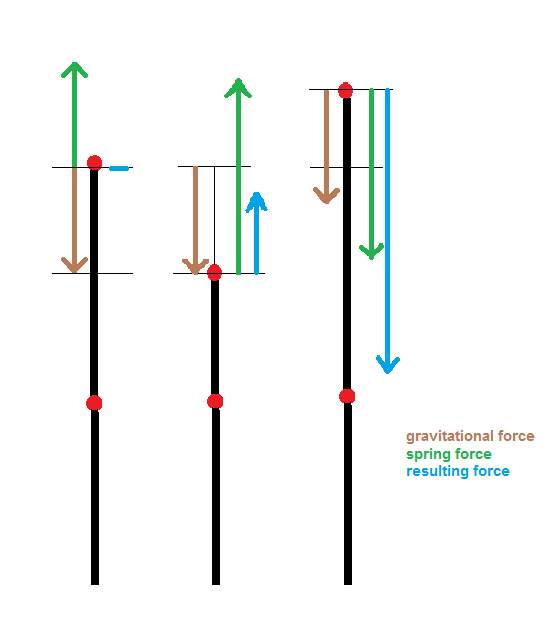
\includegraphics[width=0.8\linewidth]{SpringForce.png}
}
\caption{Spring force}
\end{figure}

\begin{figure}[htbp]
\centering
\fbox{
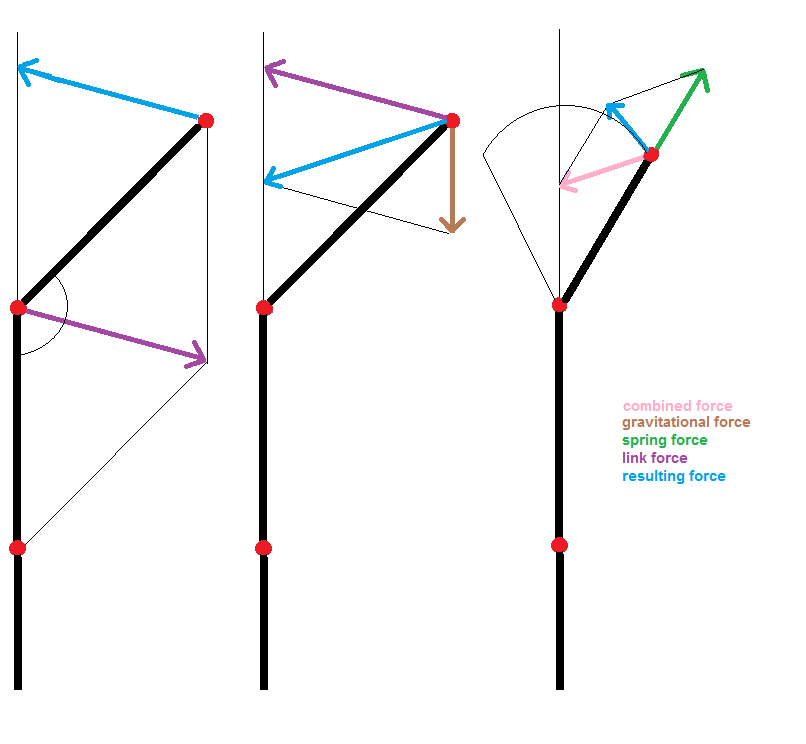
\includegraphics[width=0.8\linewidth]{CombinedForce.png}
}
\caption{Combination of all forces}
\end{figure}


\subsubsection{Wind}
wind force \\ control direction and intensity (maximum force and interval)


\section{Implementation}
The sumulation is implemented in C++ and OpenCL. There are classes for the needed data types: \textit{Vector}, \textit{Node}, \textit{Link} and \textit{HairPiece}. These classes need to have a representation in OpenCL data types. This is trivial for the vector which is a single float3. The other classes have methods to convert instances to OpenCL compatible data types.

The classes \textit{clHelper} and \textit{BodySolver} are the connection to OpenCL, they include simple helper functions and the simulation scheduling for the GPU. \textit{BodySolverCPU} is still present in the repository but not used; it is the CPU implementation of the simulation being used as the template for the implementation in OpenCL. The class \textit{GLwindow} contains the initialization of the window in OpenGL.

\subsection{Classes}
\begin{figure}[!h]
\centering
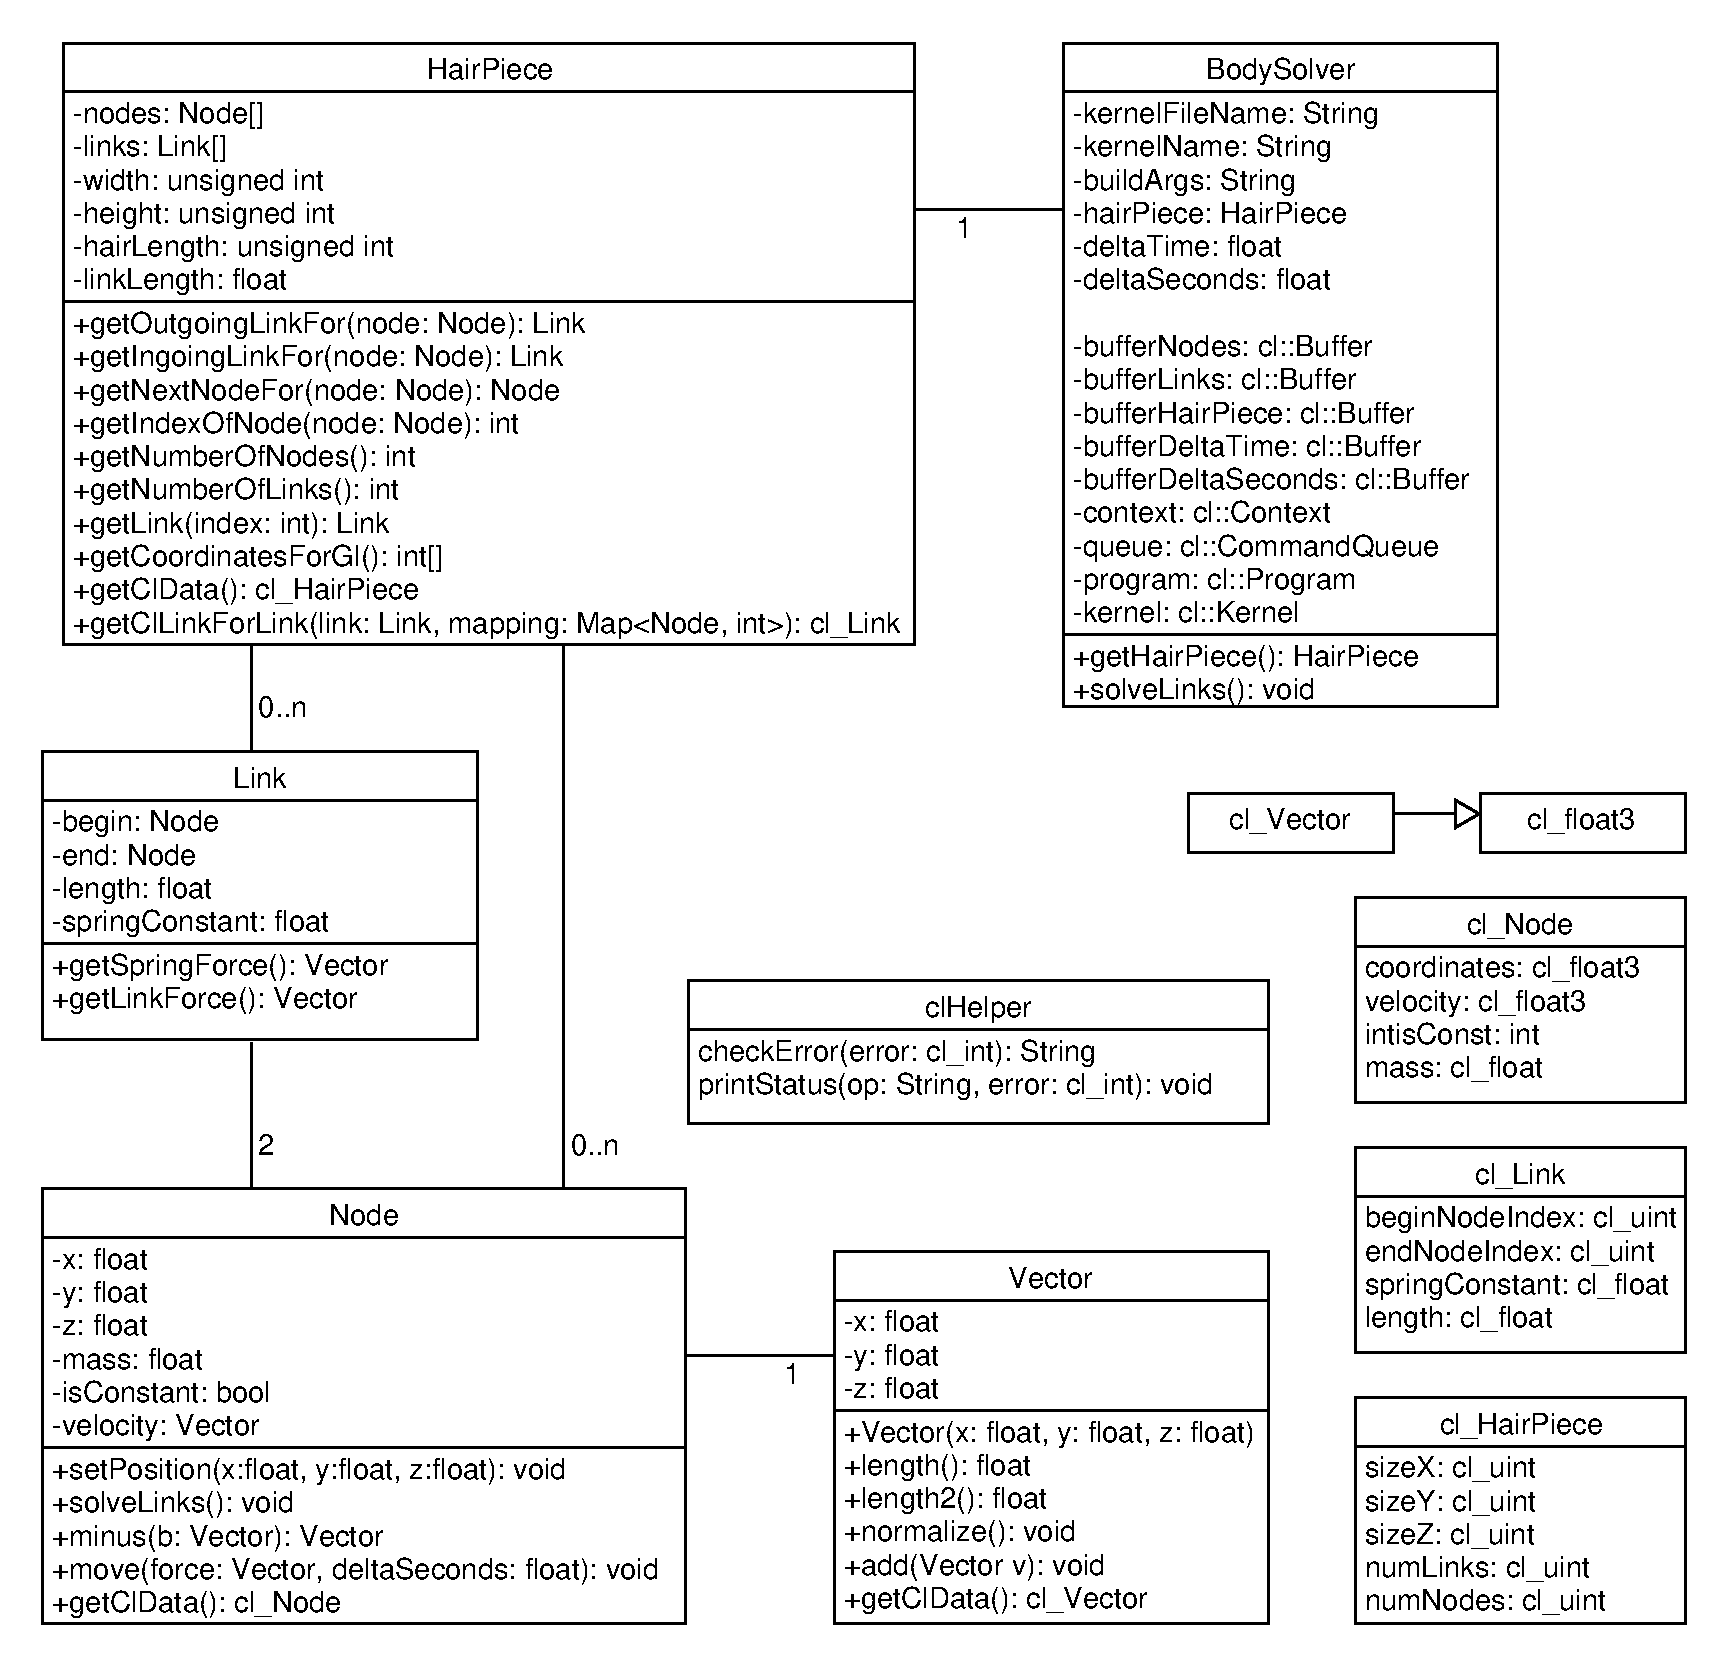
\includegraphics[width=0.8\linewidth]{Classes.pdf}
\caption{Class diagram}
\end{figure}

\subsubsection{Vector}
This is a class representating a vector in 3D space. It implements some operators like addition (with vector or scalar), length calculation and normalization.
It is used to represent forces, movement and velocities of the nodes.

\subsubsection{Node}
It represents a node of a hair, so it has a position in 3D space, mass, velocity (as Vector class) and may be constant. If it is constant it is prevented from moving, so one side of the hair nodes can be constant so that this side is assumed to be on the surface of another object.

\subsubsection{Link}
This is a link between two nodes and so has 4 elements: one node at each side, the length and a spring constant.

The Spring force is calculated with the distance from the two nodes, the difference o this length to the original link length and the spring constant.

\subsubsection{HairPiece}
HairPiece is a container class for all hairs that belong to one object. It contains a vector with all nodes and one vector with all links.

\subsubsection{clHelper}
This class contains two helper functions to decode OpenCL error codes and print status messages.

\subsubsection{BodySolver}
This class implements the handling of the OpenCL kernel implementing the actual simulation. \textit{BodySolver} contains the nodes and links of the hairs in a \textit{HairPiece} object. The Buffers for copying the nodes and links are created in the constructor, the kernel is compiled there too.

For each time step BodySolver calls the kernel; before that, the nodes and links are converted from CPU data types to OpenCL data thyes and copied to the device. Then the kernel is called, calculated the new positions forces and position of the nodes. Then the nodes are copied back and being converted back to CPU data types. Then the hairs are going to be re-drawn.

\subsubsection{GLwindow}



\subsection{Architecture}

\subsection{OpenCL}
The general flow of the program is as follows and will be discussed in this section:
\begin{enumerate}
	\item List all OpenCL platforms with GPU devices and major version 1 (or 2 alternatively)
	\item Select platform according to the preffered vendor list below
	\item Create OpenCL context and command queue for the first device of the chosen platform
	\item Create BodySolver with context and command queue and for each time step:
	\begin{enumerate}
		\item Copy nodes and links to GPU device
		\item Calculate new positions of the nodes according to the forces
		\item Copy nodes back to host
		\item Render nodes and links
	\end{enumerate}
\end{enumerate}

In the main method the platform for OpenCL is selected. The platform must contain at least one GPU device, the OpenCL version 1.* is preferred over version 2.*. For the case that multiple platform with GPUs and the same major version exist there is a list of preferred manufacturers. The list is in reverse order, so from multiple platform the lower most platform is chosen:
\begin{itemize}
	\item Intel(R) Corporation
	\item NVIDIA Corporation
	\item Advanced Micro Devices, Inc.
\end{itemize}
If no platform is found the program aborts with -1. In the console output the found and chosen platforms will be printed.

For the selected platform a context with the GPU devies is created. Then a list of GPU devies is queried from that context. For the device a command queue is created. Then the \textit{BodySolver} can be created with the context and command queue. The \textit{BodySover} calculates the new position of the nodes for each time step.

For each time step the data (nodes, links) are copied to the GPU device, then the new positions are calculated, and the data is copied back to be displayed by the \textit{GLwindow} class. This is quite inefficient because for the nodes and links to be rendered they must be copied to the GPU again. It would be more efficient to use the OpenCL extension for interopability with OpenGL.

\subsection{OpenGL}


\section{Building}
The program can be built by importing the HairSimulation.sln in Visual Studio 2017 and then builing all sub-projects.

To run the program several files must be copied in the folder where the executable is located: The two shaders in \verb|HairSim\OpenCLProject1\Sample\shader| (fragment.glsl and vertex.glsl) must be places in the same diretory as the executable HairSim.exe. The OpenCL kernel SolvePositionsFromLinksKernel.cl must also be present, but should be copied from Visual Stuidio while building.


\section{Conclusion}


An improvement would be to use the OpenCL extension for interoperation with OpenCL. This would reduce the cost of copying the nodes back and forth from and to the CPU. With the interoperability the data could reside only in the GPU's memory. The only reason to copy the data to the CPU would be to persist it to the disk.


\end{document}